

\tikzset{every picture/.style={line width=0.75pt}} %set default line width to 0.75pt        

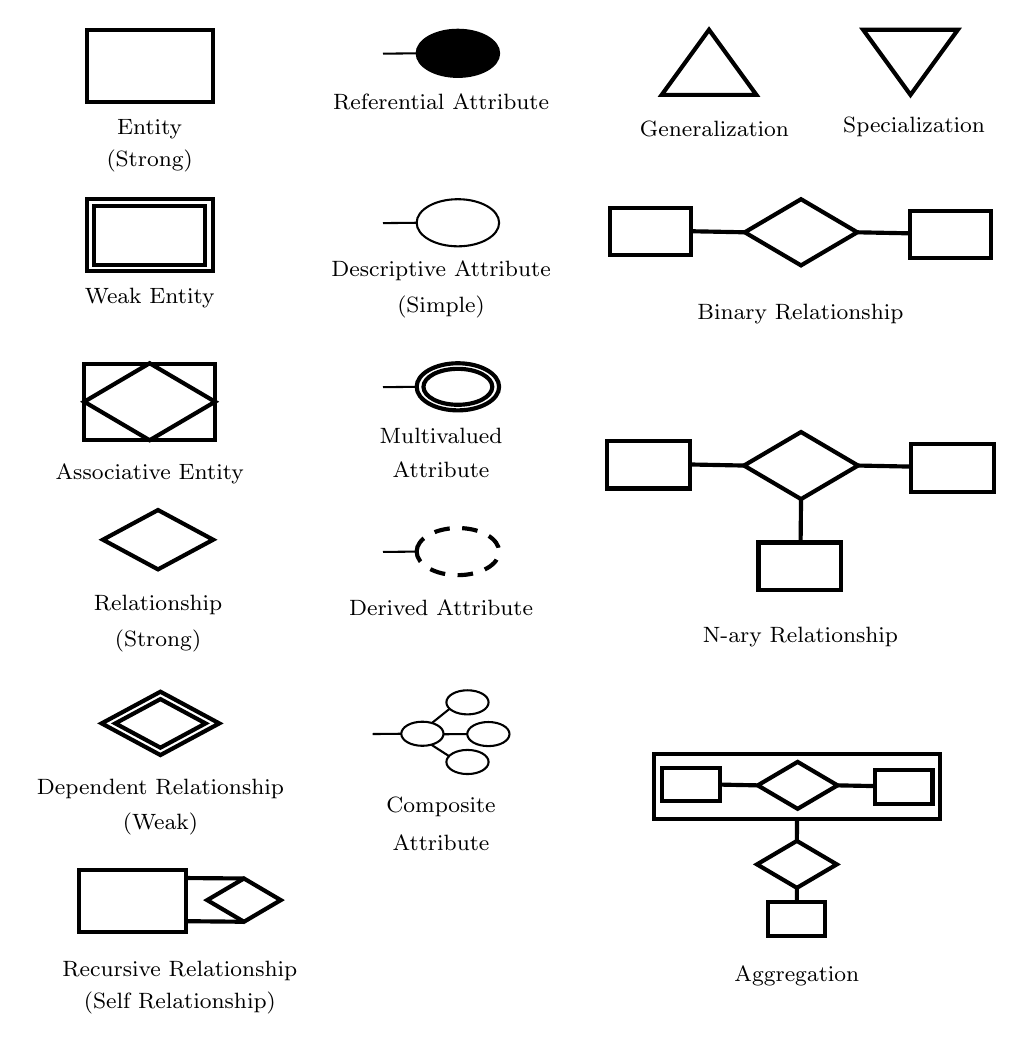
\begin{tikzpicture}[x=0.65pt,y=0.65pt,yscale=-1,xscale=1]
%uncomment if require: \path (0,597); %set diagram left start at 0, and has height of 597

%Shape: Rectangle [id:dp9409938961254447] 
\draw  [line width=1.5]  (29,15) -- (99,15) -- (99,55) -- (29,55) -- cycle ;

%Shape: Rectangle [id:dp25825363492065057] 
\draw  [line width=1.5]  (29,109.2) -- (99,109.2) -- (99,149.2) -- (29,149.2) -- cycle ;
%Shape: Rectangle [id:dp9273607878616594] 
\draw  [line width=1.5]  (33.2,112.8) -- (94.8,112.8) -- (94.8,145.6) -- (33.2,145.6) -- cycle ;

%Shape: Diamond [id:dp07590485693463012] 
\draw  [line width=1.5]  (68.65,282) -- (99.3,298.5) -- (68.65,315) -- (38,298.5) -- cycle ;

%Shape: Diamond [id:dp8393196312653484] 
\draw  [line width=1.5]  (70,383) -- (102.71,400.61) -- (70,418.22) -- (37.29,400.61) -- cycle ;
%Shape: Diamond [id:dp11016744869268091] 
\draw  [line width=1.5]  (70,387.11) -- (95.08,400.61) -- (70,414.11) -- (44.92,400.61) -- cycle ;

%Shape: Ellipse [id:dp8577075014649969] 
\draw   (212.43,122.3) .. controls (212.43,115.07) and (222.69,109.2) .. (235.35,109.2) .. controls (248.01,109.2) and (258.28,115.07) .. (258.28,122.3) .. controls (258.28,129.53) and (248.01,135.4) .. (235.35,135.4) .. controls (222.69,135.4) and (212.43,129.53) .. (212.43,122.3) -- cycle ;
%Straight Lines [id:da240419684606217] 
\draw    (193.72,122.5) -- (212.43,122.3) ;


%Shape: Ellipse [id:dp11655523259938039] 
\draw  [fill={rgb, 255:red, 0; green, 0; blue, 0 }  ,fill opacity=1 ] (212.43,28.1) .. controls (212.43,20.87) and (222.69,15) .. (235.35,15) .. controls (248.01,15) and (258.28,20.87) .. (258.28,28.1) .. controls (258.28,35.33) and (248.01,41.2) .. (235.35,41.2) .. controls (222.69,41.2) and (212.43,35.33) .. (212.43,28.1) -- cycle ;
%Straight Lines [id:da7122954732701139] 
\draw    (193.72,28.3) -- (212.43,28.1) ;


%Shape: Ellipse [id:dp23076223718363464] 
\draw  [line width=1.5]  (212.43,213.5) .. controls (212.43,206.27) and (222.69,200.4) .. (235.35,200.4) .. controls (248.01,200.4) and (258.28,206.27) .. (258.28,213.5) .. controls (258.28,220.74) and (248.01,226.6) .. (235.35,226.6) .. controls (222.69,226.6) and (212.43,220.74) .. (212.43,213.5) -- cycle ;
%Straight Lines [id:da42071644925844054] 
\draw    (193.72,213.7) -- (212.43,213.5) ;
%Shape: Ellipse [id:dp409593727665448] 
\draw  [line width=1.5]  (216.22,213.5) .. controls (216.22,207.99) and (224.78,203.51) .. (235.35,203.51) .. controls (245.92,203.51) and (254.48,207.99) .. (254.48,213.5) .. controls (254.48,219.02) and (245.92,223.49) .. (235.35,223.49) .. controls (224.78,223.49) and (216.22,219.02) .. (216.22,213.5) -- cycle ;


%Shape: Ellipse [id:dp12298573968430726] 
\draw   (203.9,406.37) .. controls (203.9,402.67) and (209.15,399.67) .. (215.63,399.67) .. controls (222.11,399.67) and (227.36,402.67) .. (227.36,406.37) .. controls (227.36,410.07) and (222.11,413.07) .. (215.63,413.07) .. controls (209.15,413.07) and (203.9,410.07) .. (203.9,406.37) -- cycle ;
%Straight Lines [id:da026255036427652145] 
\draw    (187.96,406.53) -- (203.9,406.37) ;
%Shape: Ellipse [id:dp035873659384954015] 
\draw   (228.96,388.9) .. controls (228.96,385.2) and (234.21,382.2) .. (240.69,382.2) .. controls (247.17,382.2) and (252.42,385.2) .. (252.42,388.9) .. controls (252.42,392.61) and (247.17,395.61) .. (240.69,395.61) .. controls (234.21,395.61) and (228.96,392.61) .. (228.96,388.9) -- cycle ;
%Straight Lines [id:da0884897826197295] 
\draw    (220.87,400.43) -- (230.56,392.66) ;
%Shape: Ellipse [id:dp33703819371371857] 
\draw   (240.57,406.54) .. controls (240.57,402.84) and (245.83,399.84) .. (252.31,399.84) .. controls (258.78,399.84) and (264.04,402.84) .. (264.04,406.54) .. controls (264.04,410.24) and (258.78,413.24) .. (252.31,413.24) .. controls (245.83,413.24) and (240.57,410.24) .. (240.57,406.54) -- cycle ;
%Straight Lines [id:da041465674734754376] 
\draw    (227.45,406.65) -- (240.57,406.54) ;
%Shape: Ellipse [id:dp8994114077261279] 
\draw   (228.96,422.06) .. controls (228.96,418.36) and (234.21,415.36) .. (240.69,415.36) .. controls (247.17,415.36) and (252.42,418.36) .. (252.42,422.06) .. controls (252.42,425.77) and (247.17,428.77) .. (240.69,428.77) .. controls (234.21,428.77) and (228.96,425.77) .. (228.96,422.06) -- cycle ;
%Straight Lines [id:da5145813744043246] 
\draw    (220.73,412.57) -- (230.48,418.83) ;


%Shape: Triangle [id:dp717941434970198] 
\draw  [line width=1.5]  (374.97,15) -- (401.3,51.2) -- (348.65,51.2) -- cycle ;

%Shape: Triangle [id:dp8547281306342895] 
\draw  [line width=1.5]  (486.97,51.2) -- (460.65,15) -- (513.3,15) -- cycle ;

%Shape: Ellipse [id:dp057823722753663986] 
\draw  [dash pattern={on 5.63pt off 4.5pt}][line width=1.5]  (212.43,305.1) .. controls (212.43,297.87) and (222.69,292) .. (235.35,292) .. controls (248.01,292) and (258.28,297.87) .. (258.28,305.1) .. controls (258.28,312.33) and (248.01,318.2) .. (235.35,318.2) .. controls (222.69,318.2) and (212.43,312.33) .. (212.43,305.1) -- cycle ;
%Straight Lines [id:da4937273930595423] 
\draw    (193.72,305.3) -- (212.43,305.1) ;


%Shape: Diamond [id:dp8682093873982866] 
\draw  [line width=1.5]  (426.11,109.2) -- (457.39,127.6) -- (426.11,146) -- (394.83,127.6) -- cycle ;
%Shape: Rectangle [id:dp16263593596228687] 
\draw  [line width=1.5]  (319.8,113.94) -- (365.03,113.94) -- (365.03,140.15) -- (319.8,140.15) -- cycle ;
%Shape: Rectangle [id:dp9045715408610813] 
\draw  [line width=1.5]  (486.57,115.67) -- (531.8,115.67) -- (531.8,141.89) -- (486.57,141.89) -- cycle ;
%Straight Lines [id:da894737740624673] 
\draw [line width=1.5]    (366.09,127.03) -- (394.83,127.6) ;
%Straight Lines [id:da45477038200691244] 
\draw [line width=1.5]    (457.39,127.6) -- (486.13,128.17) ;


%Shape: Diamond [id:dp8788662265812572] 
\draw  [line width=1.5]  (426.12,238.62) -- (457.82,257.27) -- (426.12,275.92) -- (394.41,257.27) -- cycle ;
%Shape: Rectangle [id:dp7607057696775741] 
\draw  [line width=1.5]  (318.35,243.42) -- (364.2,243.42) -- (364.2,270) -- (318.35,270) -- cycle ;
%Shape: Rectangle [id:dp20655084709944105] 
\draw  [line width=1.5]  (487.4,245.18) -- (533.25,245.18) -- (533.25,271.76) -- (487.4,271.76) -- cycle ;
%Straight Lines [id:da33926375234409023] 
\draw [line width=1.5]    (365.28,256.69) -- (394.41,257.27) ;
%Straight Lines [id:da8300796405989177] 
\draw [line width=1.5]    (457.82,257.27) -- (486.95,257.85) ;
%Shape: Rectangle [id:dp11640389244166749] 
\draw  [line width=1.5]  (402.47,300.05) -- (448.32,300.05) -- (448.32,326.63) -- (402.47,326.63) -- cycle ;
%Straight Lines [id:da04160890165480735] 
\draw [line width=1.5]    (425.88,299.64) -- (426.12,275.92) ;


%Shape: Diamond [id:dp09298931741553762] 
\draw  [line width=1.5]  (116.43,486.83) -- (136.89,498.86) -- (116.43,510.89) -- (95.98,498.86) -- cycle ;
%Shape: Rectangle [id:dp7562868332770196] 
\draw  [line width=1.5]  (24.66,482.2) -- (84.33,482.2) -- (84.33,516.79) -- (24.66,516.79) -- cycle ;
%Straight Lines [id:da5257649797909345] 
\draw [line width=1.5]    (84.98,510.57) -- (116.43,510.89) ;

%Straight Lines [id:da741474729938117] 
\draw [line width=1.5]    (83.76,486.58) -- (116.43,486.83) ;

%Shape: Diamond [id:dp27975998103917443] 
\draw  [line width=1.5]  (424.23,422.01) -- (446.41,435.06) -- (424.23,448.11) -- (402.04,435.06) -- cycle ;
%Shape: Rectangle [id:dp27388026856661996] 
\draw  [line width=1.5]  (348.82,425.37) -- (380.9,425.37) -- (380.9,443.97) -- (348.82,443.97) -- cycle ;
%Shape: Rectangle [id:dp8682931511633045] 
\draw  [line width=1.5]  (467.12,426.6) -- (499.19,426.6) -- (499.19,445.2) -- (467.12,445.2) -- cycle ;
%Straight Lines [id:da8247964733470876] 
\draw [line width=1.5]    (381.66,434.65) -- (402.04,435.06) ;
%Straight Lines [id:da507174915044009] 
\draw [line width=1.5]    (446.41,435.06) -- (466.8,435.46) ;
%Shape: Diamond [id:dp489563487309699] 
\draw  [line width=1.5]  (423.82,465.94) -- (446,478.99) -- (423.82,492.04) -- (401.63,478.99) -- cycle ;
%Straight Lines [id:da8803188939906841] 
\draw [line width=1.5]    (423.85,453.98) -- (423.82,465.94) ;
%Shape: Rectangle [id:dp2462964817052231] 
\draw  [line width=1.5]  (407.53,500.09) -- (439.61,500.09) -- (439.61,518.68) -- (407.53,518.68) -- cycle ;
%Straight Lines [id:da17335151983105646] 
\draw [line width=1.5]    (423.82,492.04) -- (423.83,500.08) ;
%Shape: Rectangle [id:dp019446741600327666] 
\draw  [line width=1.5]  (344.3,417.82) -- (503.3,417.82) -- (503.3,453.62) -- (344.3,453.62) -- cycle ;


%Shape: Rectangle [id:dp7508437049659447] 
\draw  [line width=1.5]  (27.54,200.66) -- (100.46,200.66) -- (100.46,242.94) -- (27.54,242.94) -- cycle ;
%Shape: Diamond [id:dp4714864707556645] 
\draw  [line width=1.5]  (64,200.4) -- (100.38,221.8) -- (64,243.2) -- (27.62,221.8) -- cycle ;



% Text Node
\draw (64,70) node  [font=\footnotesize] [align=left] {Entity};
% Text Node
\draw (64,88) node  [font=\footnotesize] [align=left] {(Strong)};
% Text Node
\draw (64,164.2) node  [font=\footnotesize] [align=left] {Weak Entity};
% Text Node
\draw (226,55.1) node   [align=left] {{\footnotesize Referential Attribute}};
% Text Node
\draw (226,447) node  [font=\footnotesize] [align=left] {Composite};
% Text Node
\draw (226,467) node  [font=\footnotesize] [align=left] {Attribute};
% Text Node
\draw (226,149.3) node   [align=left] {{\footnotesize Descriptive Attribute}};
% Text Node
\draw (226,169.3) node   [align=left] {{\footnotesize (Simple)}};
% Text Node
\draw (68.65,334.8) node  [font=\footnotesize] [align=left] {Relationship};
% Text Node
\draw (68.65,354.8) node  [font=\footnotesize] [align=left] {(Strong)};
% Text Node
\draw (70,436.8) node  [font=\footnotesize] [align=left] {Dependent Relationship};
% Text Node
\draw (70,456.8) node  [font=\footnotesize] [align=left] {(Weak)};
% Text Node
\draw (226,240.5) node   [align=left] {{\footnotesize Multivalued}};
% Text Node
\draw (226,259.5) node   [align=left] {{\footnotesize Attribute}};
% Text Node
\draw (489,69) node  [font=\footnotesize] [align=left] {Specialization};
% Text Node
\draw (226,336.1) node   [align=left] {{\footnotesize Derived Attribute}};
% Text Node
\draw (378,70) node  [font=\footnotesize] [align=left] {Generalization};
% Text Node
\draw (425.8,352.42) node  [font=\footnotesize] [align=left] {N-ary Relationship};
% Text Node
\draw (425.8,173.22) node  [font=\footnotesize] [align=left] {Binary Relationship};
% Text Node
\draw (423.8,541.2) node  [font=\footnotesize] [align=left] {Aggregation};
% Text Node
\draw (80.78,538.2) node  [font=\footnotesize] [align=left] {Recursive Relationship};
% Text Node
\draw (80.78,556.2) node  [font=\footnotesize] [align=left] {(Self Relationship)};
% Text Node
\draw (64,262.2) node   [align=left] {{\footnotesize Associative Entity}};


\end{tikzpicture}
